\documentclass[14pt]{beamer}
\usetheme{Montpellier}
\usecolortheme{beaver}

\usepackage{amsmath, amssymb, ../../vimacros, hyperref, enumerate}
\usepackage[round]{natbib}

\hypersetup{breaklinks=true, colorlinks=true, linkcolor=blue, citecolor=blue, urlcolor=blue}

\usepackage{tikz}
\usetikzlibrary{bayesnet}
\beamertemplatenavigationsymbolsempty

\title{Variational Inference: The Basics}
\date{}
\author[Schulz and Aziz]{Philip Schulz and Wilker Aziz \\
\url{https://github.com/philschulz/VITutorial}}

\setbeamertemplate{footline}[frame number]

\begin{document}

\frame{\titlepage}

\frame{\tableofcontents}

\section{Generative Models}
\frame{\tableofcontents[currentsection]}

\begin{frame}{Joint Distribution}
Let $ X $ and $ Z $ be random variables. A generative model is any model that defines a joint distribution
over these variables. 
\pause
\begin{block}{3 Examples of Generative Models}
\begin{itemize}
\item $ p(x,z) = p(x) p(z|x) $
\item $ p(x,z) = p(z) p(x|z) $
\item $ p(x,z) = p(x) p(z) $
\end{itemize}
\end{block}
\end{frame}

\begin{frame}{Likelihood and prior}
From here on, $ x $ is our observed data. On the other hand, $ z $ is an unobserved outcome. 
\begin{itemize}
\item $ p(x|z) $ is the \textbf{likelihood}
\item $ p(z) $ is the \textbf{prior} over $ Z $
\end{itemize} 
Notice: both distributions may depend on a non-random quantity $ \alpha $ (write e.g. $ p(z|\alpha) $). In that case, we 
call $ \alpha $ a hyperparameter.
\end{frame}

\begin{frame}{Bayes rule}
We can \textit{invert} a conditional probability distribution.
\begin{equation*}
p(z|x) = \frac{p(x|z)p(z)}{p(x)}
\end{equation*}
\end{frame}

\begin{frame}{Bayes rule}
We can \textit{invert} a conditional probability distribution.
\begin{equation*}
p(z|x) = \frac{\overbrace{p(x|z)}^{\text{likelihood}}\overbrace{p(z)}^{prior}}{p(x)}
\end{equation*}
\end{frame}

\begin{frame}{Bayes rule}
We can \textit{invert} a conditional probability distribution.
\begin{equation*}
\underbrace{p(z|x)}_{\text{posterior}} = \frac{\overbrace{p(x|z)}^{\text{likelihood}}\overbrace{p(z)}^{prior}}{p(x)}
\end{equation*}
\end{frame}

\begin{frame}{Bayes rule}
We can \textit{invert} a conditional probability distribution.
\begin{equation*}
\underbrace{p(z|x)}_{\text{posterior}} = \frac{\overbrace{p(x|z)}^{\text{likelihood}}\overbrace{p(z)}^{\text{prior}}}{\underbrace{p(x)}_{\text{\alert{marginal likelihood/evidence}}}}
\end{equation*}
\end{frame}

\begin{frame}{The Basic Problem}
We want to compute the posterior over latent variables $ p(z|x) $. This involves computing the marginal likelihood
$$ p(x) = \intl{ p(x,z) }{z} $$
which is often \textbf{intractable}. This problem motivates the use of \textbf{approximate inference} techniques.
\end{frame}

%\begin{frame}{Bayesian Inference}
%Model parameters $ \theta $ are also random. The generative model becomes
%\begin{itemize}
%\item $ p(x,\theta) $ for fully observed data (supervised learning)
%\item $ p(x,z,\theta) $ for observed and latent data \\ (unsupervised learning)
%\end{itemize}
%\end{frame}
%
%\begin{frame}{Bayesian Inference}
%The evidence becomes even harder to compute because $ \theta $ is often high-dimensional
%(just think of neural nets!).
%\begin{itemize}
%\item $ p(x) = \intl{ p(x, \theta)}{\theta} $ (supervised learning)
%\item $ p(x) = \intl{ \intl{ p(x, z, \theta)} {z}}{\theta} $ (unsupervised learning)
%\end{itemize}
%\pause
%Again, approximate inference is needed.
%\end{frame}

\section{Examples}
\frame{\tableofcontents[currentsection]}

\begin{frame}{We cannot compute the posterior when}
\begin{enumerate}
\item The functional form of the posterior is unknown (we don't know which parameters to infer)
\item The functional form is known but the computation is intractable
\end{enumerate}
\end{frame}

\begin{frame}{Bayesian Log-Linear POS Tagger}
\begin{figure}
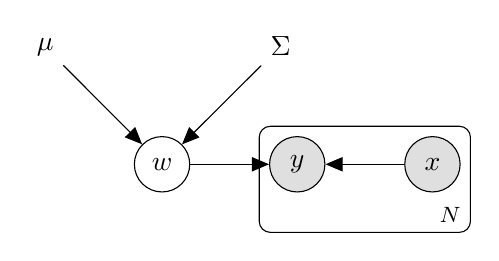
\begin{tikzpicture}
\node[obs] (x) {$ y $};
\node[latent, left=of x] (w) {$ w $};
\node[obs,right=of x] (f) {$ x $};
\plate {data} {(x)(f)} {$ N $};
\edge{w,f}{x};
\pause
\node[above left= of w] (mu) {$ \mu $};
\node[above right=of w] (sigma) {$ \Sigma $};
\edge{mu,sigma}{w};
\end{tikzpicture}
\end{figure}
The Normal distribution is not conjugate to the Gibbs distribution. The form of the posterior is unknown.
\end{frame}

\begin{frame}{Bayesian Log-Linear POS Tagger}
\begin{block}{Intuition}
Simply assume that the posterior is Gaussian.
\end{block}
\end{frame}

\begin{frame}{Factorial HMMs}
FHMMs have several Markov chains over latent variables.
\begin{figure}
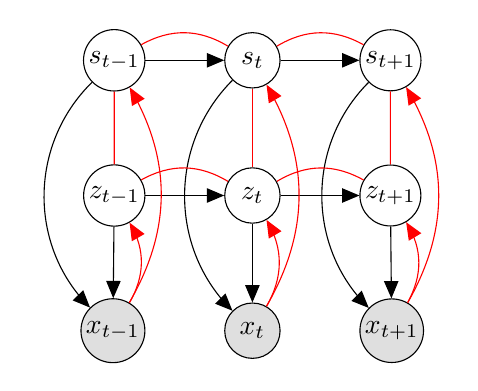
\begin{tikzpicture}
\node[obs] (xt) {$ x_{t} $};
\node[obs, left=of xt] (xt-1) {$ x_{t-1} $};
\node[obs, right=of xt] (xt+1) {$ x_{t+1} $};

\node[latent, above= of xt] (zt) {$ z_{t} $};
\node[latent, left= of zt] (zt-1) {$ z_{t-1} $};
\node[latent, right= of zt] (zt+1) {$ z_{t+1} $};

\edge {zt} {xt, zt+1};
\edge {zt-1} {xt-1, zt};
\edge {zt+1} {xt+1};

\pause
\node[latent, above= of zt] (st) {$ s_{t} $};
\node[latent, left= of st] (st-1) {$ s_{t-1} $};
\node[latent, right= of st] (st+1) {$ s_{t+1} $};

\edge {st-1} {st};
\edge {st} {st+1};

% bend edges don't work in bayesnet and need to be created by hand.
\path (st-1) edge[bend right=45, ->] (xt-1);
\path (st) edge[bend right=45, ->] (xt);
\path (st+1) edge[bend right=45, ->] (xt+1);

\pause
% inference edges
\path (xt-1) edge[->, color=red, bend right=30] (zt-1);
\path (xt) edge[->, color=red, bend right=30] (zt);
\path (xt+1) edge[->, color=red, bend right=30] (zt+1);

\path (xt-1) edge[->, color=red, bend right=30] (st-1);
\path (xt) edge[->, color=red, bend right=30] (st);
\path (xt+1) edge[->, color=red, bend right=30] (st+1);

\pause
\path (st-1) edge[-, color=red, bend left=30] (st);
\path (st) edge[-, color=red, bend left=30] (st+1);
\path (zt-1) edge[-, color=red, bend left=30] (zt);
\path (zt) edge[-, color=red, bend left=30] (zt+1);

\pause
\edge[-, color=red]{st-1}{zt-1};
\edge[-, color=red]{st}{zt};
\edge[-, color=red]{st+1}{zt+1};
\end{tikzpicture}
\end{figure}
\end{frame}

\begin{frame}{Factorial HMMs}
Inference network for FHHMs.
\begin{figure}
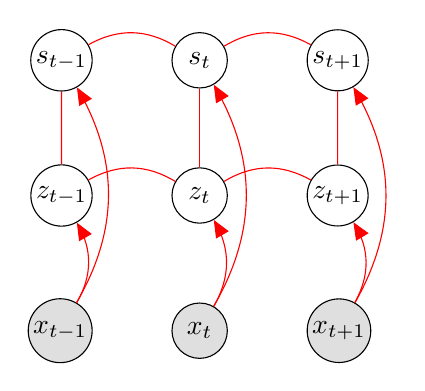
\begin{tikzpicture}
\node[obs] (xt) {$ x_{t} $};
\node[obs, left=of xt] (xt-1) {$ x_{t-1} $};
\node[obs, right=of xt] (xt+1) {$ x_{t+1} $};

\node[latent, above= of xt] (zt) {$ z_{t} $};
\node[latent, left= of zt] (zt-1) {$ z_{t-1} $};
\node[latent, right= of zt] (zt+1) {$ z_{t+1} $};

\node[latent, above= of zt] (st) {$ s_{t} $};
\node[latent, left= of st] (st-1) {$ s_{t-1} $};
\node[latent, right= of st] (st+1) {$ s_{t+1} $};

% inference edges
\path (xt-1) edge[->, color=red, bend right=30] (zt-1);
\path (xt) edge[->, color=red, bend right=30] (zt);
\path (xt+1) edge[->, color=red, bend right=30] (zt+1);

\path (xt-1) edge[->, color=red, bend right=30] (st-1);
\path (xt) edge[->, color=red, bend right=30] (st);
\path (xt+1) edge[->, color=red, bend right=30] (st+1);

\edge[-, color=red]{st-1}{zt-1};
\edge[-, color=red]{st}{zt};
\edge[-, color=red]{st+1}{zt+1};

\path (st-1) edge[-, color=red, bend left=30] (st);
\path (st) edge[-, color=red, bend left=30] (st+1);
\path (zt-1) edge[-, color=red, bend left=30] (zt);
\path (zt) edge[-, color=red, bend left=30] (zt+1);
\end{tikzpicture}
\end{figure}
\end{frame}

\begin{frame}{Factorial HMMs}
FHMMs have several Markov chains over latent variables.
\begin{itemize}
\item $ M $ Markov chains over latent variables.
\item $ L $ outcomes per latent variable.
\item Sequence of length $ T $.
\item Complexity of inference: $ \mathcal{O}(L^{2M}T) $.
\end{itemize}
\pause
\begin{alertblock}{Intractable}
Exponential dependency on the number of hidden Markov chains.
\end{alertblock}
\end{frame}

\begin{frame}{Factorial HMMs}
\begin{block}{Intuition}
Simply assume that the posterior consists of independent Markov chains.
\end{block}
\end{frame}

\begin{frame}{Latent Dirichlet Allocation}
An admixture model that changes its mixture weights per document. We assume that the mixture components
are fixed.
\begin{figure}
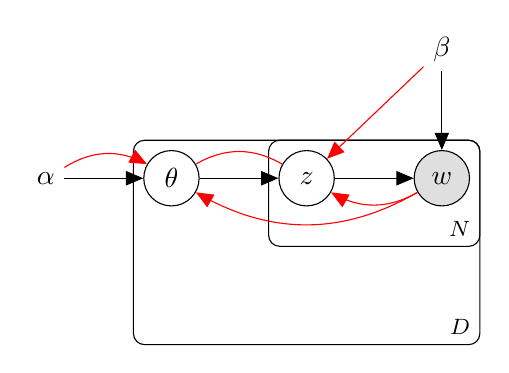
\begin{tikzpicture}
\node[obs] (w) {$ w $};
\node[latent, left= of w] (z) {$ z $};
\node[latent, left= of z] (theta) {$ \theta $};
\node[left= of theta] (alpha) {$ \alpha $};
\node[above= of w] (beta) {$ \beta $};
\node[below= of z] (fake) {}; % needed to fit the document plate

\plate {tokens} {(w)(z)} {$ N $};
\plate {document} {(w)(z)(theta)(fake)} {$ D $};

\edge {alpha} {theta};
\edge {theta} {z};
\edge {z} {w};
\edge {beta} {w};

\pause
% inference edges
\path (w) edge[->,bend left=30,color=red] (z);
\edge[color=red] {beta} {z};
\path (w) edge[->,bend left=30,color=red] (theta);
\pause
\path (z) edge[-,bend right=30,color=red] (theta);
\path (alpha) edge[->, bend left=30, color=red] (theta);
\end{tikzpicture}
\end{figure}
\end{frame}

\begin{frame}{Latent Dirichlet Allocation}
Inference network for LDA.
\begin{figure}
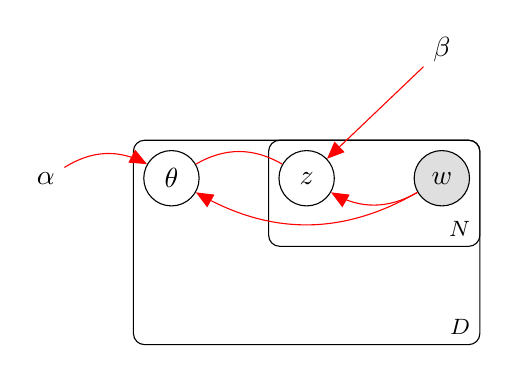
\begin{tikzpicture}
\node[obs] (w) {$ w $};
\node[latent, left= of w] (z) {$ z $};
\node[latent, left= of z] (theta) {$ \theta $};
\node[left= of theta] (alpha) {$ \alpha $};
\node[above= of w] (beta) {$ \beta $};
\node[below= of z] (fake) {}; % needed to fit the document plate

\plate {tokens} {(w)(z)} {$ N $};
\plate {document} {(w)(z)(theta)(fake)} {$ D $};

% inference edges
\path (w) edge[->,bend left=30,color=red] (z);
\path (w) edge[->,bend left=30,color=red] (theta);
\path (z) edge[-,bend right=30,color=red] (theta);
\path (alpha) edge[->, bend left=30, color=red] (theta);
\edge[color=red] {beta} {z};
\end{tikzpicture}
\end{figure}
\end{frame}

\begin{frame}{Latent Dirichlet Allocation}
An admixture model that changes its mixture weights per document. Here we assume that the mixture components
are fixed.
\begin{itemize}
\item $ D $ documents.
\item $ N $ tokens and latent variables per document.
\item $ L $ outcomes per latent variable.
\item Complexity of inference: $ \mathcal{O}(L^{DN}) $.
\end{itemize}
\end{frame}

\begin{frame}{Latent Dirichlet Allocation}
\begin{block}{Intuition}
Simply assume that the posterior consists of independent categorical and Dirichlet distributions.
\end{block}
\pause
\begin{block}{Rule of Thumb}
Simply assume that the posterior is in the same family as the prior.
\end{block}
\end{frame}


\section{Variational Inference}
\frame{\tableofcontents[currentsection]}

\begin{frame}{The Goal}
Assume $ p(z|x) $ is not computable.
\pause
\begin{block}{Idea}
Let's approximate it by an auxiliary distribution $ q(z) $ that is computable!
\end{block}
\pause
\begin{block}{Requirement}
Choose $ q(z) $ as close as possible to $ p(z|x) $ to obtain a faithful approximation.
\end{block}
\end{frame}

\begin{frame}{Recap KL divergence}
The Kullback-Leibler divergence (or relative entropy) measures the divergence of a distribution $ q $ from 
a distribution $ p $. 
\begin{itemize}
\pause
\item $ \KL{q(z)}{p(z|x)} = \intl{ q(z) \loga{\frac{q(z)}{p(z|x)}}}{z} $ (continuous)
\pause
\item $ \KL{q(z)}{p(z|x)} = \sum_{z} q(z) \loga{\frac{q(z)}{p(z|x)}} $ (discrete)
\pause
\item $ \KL{q(z)}{p(z|x)} = \E[q(z)]{\loga{\frac{q(z)}{p(z|x)}}} $ (both)
\end{itemize}
\end{frame}

%\begin{frame}{Recap KL divergence}
%Originally known as relative entropy. Read $ \KL{q(z)}{p(z)} $ as the divergence of $ p $ from $ q $ or the entropy of $ p $ relative to $ q $.
%\pause
%\begin{small}
%\begin{block}{Expand $ \KL{q}{p} $}
%\begin{align*}
%\E[q(z)]{\loga{\frac{q(z)}{p(z)}}} &= - \E[q(z)]{\log p(z)} + \E[q(z)]{\log q(z)} \\
%&\onslide<3->{= \text{CE} - \Ent{q(z)}}
%\end{align*}
%\end{block}
%\onslide<4>
%\end{small}
%Bits needed to encode $ p $ once we know $ q $. 
%\end{frame}

\begin{frame}{Recap KL divergence}
\begin{block}{Properties}
\begin{itemize}
\item $ \KL{q(z)}{p(z|x)} \geq 0 $ with \\ equality iff $ q(z) = p(z|x) $.
\pause
\item $ -\KL{q(z)}{p(z|x)} = \E[q(z)]{\loga{\frac{p(z|x)}{q(z)}}} \leq 0 $.
\pause
\item $ \KL{q(z)}{p(z|x)} = \infty $ \\ if $ \exists z $ s.t. $ p(z|x) = 0 $ and $ q(z) > 0 $.
%\pause
%\item In general $ \KL{q(z)}{p(z|x)} \not = \KL{p(z|x)}{q(z)} $.
\end{itemize}
\end{block}
\end{frame}

\subsection{Deriving VI with Jensen's Inequality}

\begin{frame}{VI derivation I}
\begin{small}
\begin{equation*}
\begin{aligned}
\log p(x) &= \loga{\intl{p(x,z)}{z}} \\
\pause
&= \loga{\intl{\alert{q(z)}\frac{p(x,z)}{\alert{q(z)}}}{z}} \\
\pause
&= \loga{\E[q(z)]{\frac{p(x,z)}{\alert{q(z)}}}} \\
&\geq \E[q(z)]{  \loga{\frac{p(x,z)}{\alert{q(z)}}}} \\
\pause
& = \E[q(z)] {\loga{\frac{p(z|x)p(x)}{\alert{q(z)}}}}
\end{aligned}
\end{equation*}
\end{small}
\end{frame}

\begin{frame}{VI derivation I}
\begin{equation*}
\begin{aligned}
\log p(x) &\geq 
\E[q(z|x)] {\loga{\frac{p(z|x)p(x)}{q(z)}}} \\
\pause
&= \intl{ q(z) \loga{\frac{p(z|x)}{q(z)}}}{z} + \log p(x) \\
\pause
&= -\KL{q(z)}{p(z|x)} + \log p(x)
\end{aligned}
\end{equation*}
\pause
We have derived a lower bound on the log-evidence whose gap is exactly $ \KL{q(z)}{p(z|x)} $.
\end{frame}

\subsection{Deriving VI from KL Divergence}

\begin{frame}{VI derivation II}
Recall that we want to find $ q(z) $ such that $ \KL{q(z)}{p(z|x)} $ is small.
\pause
\begin{block}{Formal Objective}
\begin{equation*}
\underset{q(z)}{\min} \KL{q(z)}{p(z|x)} \pause = \underset{q(z)}{\max} -\KL{q(z)}{p(z|x)}
\end{equation*}
\end{block}
\end{frame}

\begin{frame}{VI derivation II}
\begin{small}
\begin{equation*}
\begin{aligned}
&\underset{q(z)}{\max} -\KL{q(z)}{p(z|x)} \\ 
\pause
&= \underset{q(z)}{\max} \intl{ q(z) \loga{\frac{p(z|x)}{q(z)}}}{z} \\
\pause
&= \underset{q(z)}{\max} \intl{ q(z) \loga{\frac{p(z,x)}{p(x)q(z)}}} {z} \\
\pause
&= \underset{q(z)}{\max} \intl{ q(z) \loga{p(z,x)}} {z} - \intl{ q(z) \log q(z)} {z} 
- \overbrace{\log p(x)}^{constant} \\
\pause
&= \underset{q(z)}{\max}~\E[q(z)]{\log p(x,z) } + \Ent{q(z)}
\end{aligned}
\end{equation*}
\end{small}
\end{frame}

\begin{frame}
As before, we have derived a lower bound on the log-evidence. This \textbf{evidence lower bound}
or \textbf{ELBO} is our optimisation objective.
\begin{block}{ELBO}
\center
\boxed{
\underset{q(z)}{\max}~\E[q(z)]{\log p(x,z)} + \Ent{q(z)}
}
\end{block}
\end{frame}

\subsection{Relationship to EM}

\begin{frame}{Performing VI (Frequentist Case)}
VI in its basic form can be performed via coordinate ascent. This can be done as a 2-step procedure.
\begin{enumerate}
\pause
\item Maximize (regularised) expected log-density.
\begin{equation*}
\underset{q(z)}{\max}~\E[q(z)]{\loga{p(x,z)}} + \Ent{q(z)}
\end{equation*}
\pause
\item Optimise generative model.
\begin{equation*}
\underset{p(x,z)}{\max}~ \E[q(z)]{\loga{p(x,z)}} + \underbrace{\Ent{q(z)}}_{\text{constant}}
\end{equation*}
\end{enumerate}
\end{frame}

\begin{frame}{Recap: EM Algorithm}
\begin{itemize}
\item[\alert{E-step}] Compute: $ \E[p(z|x)]{\loga{p(x,z)}} $. \\ Same as: $ \underset{p(z|x)}{\max}~ \E[p(z|x)]{\log p(x,z)} $ \pause
\item[\alert{M-step}] $ \underset{p(x,z)}{\max}~\E[p(z|x)]{\log p(x,z)} + \underbrace{\Ent{p(z|x)}}_{\text{constant}} $
\end{itemize}
\pause 
\begin{block}{EM is variational inference!}
\begin{align*}
&q(z) = p(z|x) \\
&\KL{q(z)}{p(z|x)} = 0
\end{align*}
\end{block}
\end{frame}


%\subsection{Variational Bayes}
%
%\begin{frame}{Performing VI (Bayesian Case)}
%We have latent variables $ z $ (e.g. POS tags) and $ \theta $ (e.g. model parameters).
%\begin{enumerate}
%\item Maximise over local variables $ z $.
%\begin{equation*}
%\underset{q(z)}{\max}~\E[q(z)q(\theta)]{\log p(x,z,\theta)} + \Ent{q(z)}
%\end{equation*}
%\pause
%\item Maximise over global variables $ \theta $.
%\begin{equation*}
%\underset{q(\theta)}{\max}~ \E[q(z)q(\theta)]{\log p(x,z,\theta)} + \Ent{q(\theta)}
%\end{equation*}
%\end{enumerate}
%\end{frame}
%
%\begin{frame}{Differences between frequentist VI and VB (Variational Bayes)}
%\begin{itemize}
%\item Frequentist VI optimises two sets of parameters, VB only optimises variational parameters
%\item Entropy term matters in the M-step for VB but not for VI
%\end{itemize}
%\end{frame}

\section{Mean Field Inference}
\frame{\tableofcontents[currentsection]}

\begin{frame}{Designing a tractable approximation}
\begin{itemize}
\item Recall: The approximation $ q(z) $ needs to be tractable.
\item Common solution: make \textbf{all} latent variables independent under $ q(z) $.
\pause
\item Formal assumption: $ q(z) = \prod_{i=1}^{N}q(z_{i}) $
\end{itemize}
\pause
This approximation strategy is commonly known as \textbf{mean field} approximation.
\end{frame}





%%%%%%%%%%%%%%%%%%%%%%%%%%%%%%%%%%%%%%%%%%%%%%%


\begin{frame}{Original FHHM Inference} 
\begin{figure}
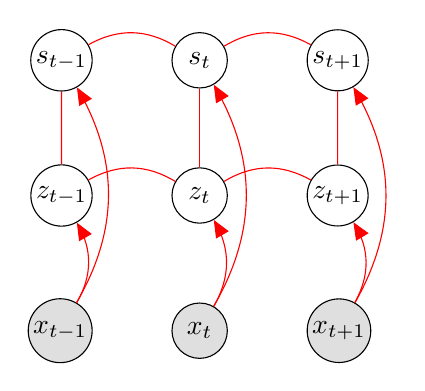
\begin{tikzpicture}
\node[obs] (xt) {$ x_{t} $};
\node[obs, left=of xt] (xt-1) {$ x_{t-1} $};
\node[obs, right=of xt] (xt+1) {$ x_{t+1} $};

\node[latent, above= of xt] (zt) {$ z_{t} $};
\node[latent, left= of zt] (zt-1) {$ z_{t-1} $};
\node[latent, right= of zt] (zt+1) {$ z_{t+1} $};

\node[latent, above= of zt] (st) {$ s_{t} $};
\node[latent, left= of st] (st-1) {$ s_{t-1} $};
\node[latent, right= of st] (st+1) {$ s_{t+1} $};

% inference edges
\path (xt-1) edge[->, color=red, bend right=30] (zt-1);
\path (xt) edge[->, color=red, bend right=30] (zt);
\path (xt+1) edge[->, color=red, bend right=30] (zt+1);

\path (xt-1) edge[->, color=red, bend right=30] (st-1);
\path (xt) edge[->, color=red, bend right=30] (st);
\path (xt+1) edge[->, color=red, bend right=30] (st+1);

\edge[-, color=red]{st-1}{zt-1};
\edge[-, color=red]{st}{zt};
\edge[-, color=red]{st+1}{zt+1};

\path (st-1) edge[-, color=red, bend left=30] (st);
\path (st) edge[-, color=red, bend left=30] (st+1);
\path (zt-1) edge[-, color=red, bend left=30] (zt);
\path (zt) edge[-, color=red, bend left=30] (zt+1);
\end{tikzpicture}
\end{figure}
\center{Exact posterior $ p(s,z|x) $}
\end{frame}

\begin{frame}{Mean field FHHM Inference}
\begin{figure}
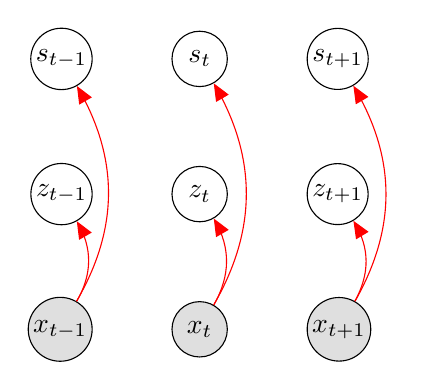
\begin{tikzpicture}
\node[obs] (xt) {$ x_{t} $};
\node[obs, left=of xt] (xt-1) {$ x_{t-1} $};
\node[obs, right=of xt] (xt+1) {$ x_{t+1} $};

\node[latent, above= of xt] (zt) {$ z_{t} $};
\node[latent, left= of zt] (zt-1) {$ z_{t-1} $};
\node[latent, right= of zt] (zt+1) {$ z_{t+1} $};

\node[latent, above= of zt] (st) {$ s_{t} $};
\node[latent, left= of st] (st-1) {$ s_{t-1} $};
\node[latent, right= of st] (st+1) {$ s_{t+1} $};

% inference edges
\path (xt-1) edge[->, color=red, bend right=30] (zt-1);
\path (xt) edge[->, color=red, bend right=30] (zt);
\path (xt+1) edge[->, color=red, bend right=30] (zt+1);

\path (xt-1) edge[->, color=red, bend right=30] (st-1);
\path (xt) edge[->, color=red, bend right=30] (st);
\path (xt+1) edge[->, color=red, bend right=30] (st+1);
\end{tikzpicture}
\end{figure}
\center{Approximate posterior $ q(s,z) = \prod_{t=1}^{T}q(s_{t})q(z_{t})$}
\end{frame}

\begin{frame}{Original LDA Inference}
\begin{figure}
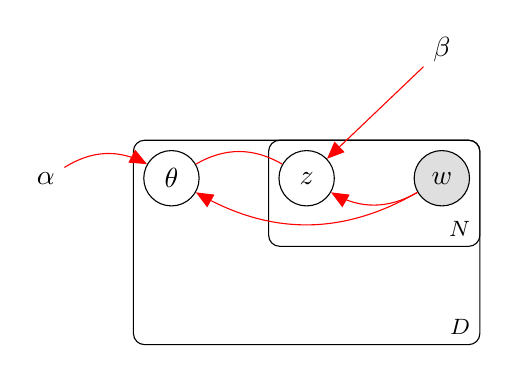
\begin{tikzpicture}
\node[obs] (w) {$ w $};
\node[latent, left= of w] (z) {$ z $};
\node[latent, left= of z] (theta) {$ \theta $};
\node[left= of theta] (alpha) {$ \alpha $};
\node[above= of w] (beta) {$ \beta $};
\node[below= of z] (fake) {}; % needed to fit the document plate

\plate {tokens} {(w)(z)} {$ N $};
\plate {document} {(w)(z)(theta)(fake)} {$ D $};

% inference edges
\path (w) edge[->,bend left=30,color=red] (z);
\path (w) edge[->,bend left=30,color=red] (theta);
\path (z) edge[-,bend right=30,color=red] (theta);
\path (alpha) edge[->, bend left=30, color=red] (theta);
\edge[color=red] {beta} {z};
\end{tikzpicture}
\end{figure}
\center{Exact posterior $ p(z,\theta|w,\alpha, \beta) $}
\end{frame}

\begin{frame}{Mean field LDA Inference}
\begin{figure}
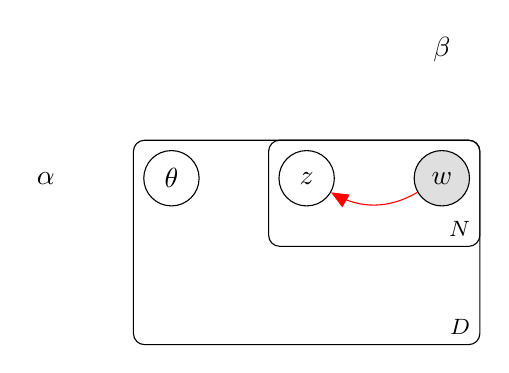
\begin{tikzpicture}
\node[obs] (w) {$ w $};
\node[latent, left= of w] (z) {$ z $};
\node[latent, left= of z] (theta) {$ \theta $};
\node[left= of theta] (alpha) {$ \alpha $};
\node[above= of w] (beta) {$ \beta $};
\node[below= of z] (fake) {}; % needed to fit the document plate

\plate {tokens} {(w)(z)} {$ N $};
\plate {document} {(w)(z)(theta)(fake)} {$ D $};

% inference edges
\path (w) edge[->,bend left=30,color=red] (z);
\end{tikzpicture}
\end{figure}
\center{Approximate posterior $ q(z,\theta|w,\alpha, \beta) = \prod_{d=1}^{D}q(\theta_{d})\prod_{i=1}^{N}q(z_i|w) $}
\end{frame}



\begin{frame}{Latent Factor Document Model}
Let us consider a latent factor model for document modelling: \pause

\begin{itemize}
	\item a document $ x = (x_{1},\ldots,x_{N})$ consists of $ n $ i.i.d. categorical draws from that model \pause
	\item the categorical distribution in turn depends on binary latent factors $ z = (z_{1},\ldots,z_{K}) $ which are also i.i.d. \pause
\end{itemize}

\begin{equation*}
\begin{aligned}
Z_{j} &\sim \Bernoulli(\alpha) && (1 \leq j \leq K) \\ 
X_{i}|z &\sim \CatDist{f_\theta(z)} && (1 \leq i \leq N)
\end{aligned}
\end{equation*} 
$ f_\theta(\cdot) $ is computed by a NN with softmax output.
\end{frame}

\begin{frame}{Original LFDM Inference}
\textcolor{blue}{Joint distribution:} latent variables are marginally independent a priori\\
$$\text{for example, }K=3, N=4$$
\begin{figure}
\center
\begin{tikzpicture}
\foreach \x in {1,...,4} {
  \pgfmathtruncatemacro{\y}{\x-1}
  \ifthenelse{\x=1}{\node[obs] (x\x) {$ x_{\x} $}}{\node[obs, right= of x\y] (x\x) {$ x_{\x} $}};
}
\foreach \z in {1,2,3} {
  \node[latent, above right = of x\z] (z\z) {$ z_{\z} $};
  \only<1>{\edge[blue]{z\z}{x1,x2,x3,x4};}
}
\foreach \z in {1,2,3} {
  \only<2>{\edge[red]{x1,x2,x3,x4}{z\z};}
}
\uncover<2->{
\edge[-,red]{z1}{z2};
\edge[-,red,bend left]{z1}{z3};
\edge[-,red]{z2}{z3};
}
\end{tikzpicture}
\end{figure}

~

\uncover<2>{\alert{Posterior: } latent variables are marginally dependent given observations}

%At inference time the latent variables are marginally dependent. For our variational distribution
%we are going to assume that they are not (recall: mean field assumption).
\end{frame}



\begin{frame}{Mean field assumption}

We have $K$ latent variables\\
\begin{itemize}
	\item assume the posterior factorises as $K$ independent terms
\end{itemize}


\begin{equation*}
q(z_1, \ldots, z_K) = \underbrace{\prod_{j=1}^K q_{\alert{\lambda_j}}(z_j)}_{\text{mean field}}
\end{equation*} \pause

with independent sets of parameters $\lambda_j = \{b_j\}$
$$Z_j \sim \Bernoulli(b_j)$$

\end{frame}

\begin{frame}{Mean field: example}
\begin{figure}
\center
\begin{tikzpicture}
\foreach \x in {1,...,4} {
\pgfmathtruncatemacro{\y}{\x-1}
\ifthenelse{\x=1}{\node[obs] (x\x) {$ x_{\x} $}}{\node[obs, right= of x\y] (x\x) {$ x_{\x} $}};
}
\foreach \z in {1,2,3} {
  \node[latent, above right = of x\z] (z\z) {$ z_{\z} $};
  \edge[color=red]{x1,x2,x3,x4}{z\z};
  \node[above = of z\z] (lambda\z) {$ \lambda_{\z} $};
  \edge[color=red]{lambda\z}{z\z};
}
\end{tikzpicture}
\end{figure}

\end{frame}


\begin{frame}{Amortised variational inference}

Amortise the cost of inference using NNs
\begin{equation*}
q(z_1, \ldots, z_K|x) = \prod_{j=1}^K q_{\alert{\lambda}}(z_j|x)
\end{equation*} \pause
~ still mean field
$$Z_j|x \sim \Bernoulli(b_j)$$\\  \pause
~ but with a shared set of parameters
\begin{itemize}
	\item where $b_1^K = g_{\alert{\lambda}}(x)$ 
\end{itemize}

\end{frame}


\begin{frame}{Amortised VI: example}
\begin{figure}
\center
\begin{tikzpicture}
\foreach \x in {1,...,4} {
\pgfmathtruncatemacro{\y}{\x-1}
\ifthenelse{\x=1}{\node[obs] (x\x) {$ x_{\x} $}}{\node[obs, right= of x\y] (x\x) {$ x_{\x} $}};
}
\foreach \z in {1,2,3} {
  \node[latent, above right = of x\z] (z\z) {$ z_{\z} $};
  \edge[color=red]{x1,x2,x3,x4}{z\z};
}
\node[above = of z2] (lambda) {$ \lambda $};
\foreach \z in {1,2,3} {
  \edge[color=red]{lambda}{z\z};
}
\end{tikzpicture}
\end{figure}

\end{frame}

\begin{frame}[plain]{Overview}

	\begin{minipage}[b][.35\textheight][t]{.47\textwidth}
	Joint\,distribution
	
	\vspace{10pt}
	
	\scalebox{0.9}{
	\begin{tikzpicture}
	\foreach \x in {1,...,4} {
	  \pgfmathtruncatemacro{\y}{\x-1}
	  \ifthenelse{\x=1}{\node[obs] (x\x) {$ x_{\x} $}}{\node[obs, right= of x\y] (x\x) {$ x_{\x} $}};
	}
	\foreach \z in {1,2,3} {
	  \node[latent, above right = of x\z] (z\z) {$ z_{\z} $};
	  \edge[blue]{z\z}{x1,x2,x3,x4};
	}
	\end{tikzpicture}}
	\end{minipage}\hfill%
    \begin{minipage}[b][.35\textheight][t]{.47\textwidth}
    Posterior
    \scalebox{0.9}{
    \begin{tikzpicture}
	\foreach \x in {1,...,4} {
	  \pgfmathtruncatemacro{\y}{\x-1}
	  \ifthenelse{\x=1}{\node[obs] (x\x) {$ x_{\x} $}}{\node[obs, right= of x\y] (x\x) {$ x_{\x} $}};
	}
	\foreach \z in {1,2,3} {
	  \node[latent, above right = of x\z] (z\z) {$ z_{\z} $};
	  \edge[red]{x1,x2,x3,x4}{z\z};
	}
	\edge[-,red]{z1}{z2};
	\edge[-,red,bend left]{z1}{z3};
	\edge[-,red]{z2}{z3};
	\end{tikzpicture}
    }
    \end{minipage}\\[0.5em]
    \begin{minipage}[b][.35\textheight][t]{.47\textwidth}
    Mean\,field
    \scalebox{0.9}{
	\begin{tikzpicture}
	\foreach \x in {1,...,4} {
	\pgfmathtruncatemacro{\y}{\x-1}
	\ifthenelse{\x=1}{\node[obs] (x\x) {$ x_{\x} $}}{\node[obs, right= of x\y] (x\x) {$ x_{\x} $}};
	}
	\foreach \z in {1,2,3} {
	  \node[latent, above right = of x\z] (z\z) {$ z_{\z} $};
	  \edge[color=red]{x1,x2,x3,x4}{z\z};
	  \node[above = of z\z] (lambda\z) {$ \lambda_{\z} $};
	  \edge[color=red]{lambda\z}{z\z};
	}
	\end{tikzpicture}}
    \end{minipage}\hfill
    \begin{minipage}[b][.35\textheight][t]{.47\textwidth}
    Amortised\,VI
    \scalebox{0.9}{
	\begin{tikzpicture}
	\foreach \x in {1,...,4} {
	\pgfmathtruncatemacro{\y}{\x-1}
	\ifthenelse{\x=1}{\node[obs] (x\x) {$ x_{\x} $}}{\node[obs, right= of x\y] (x\x) {$ x_{\x} $}};
	}
	\foreach \z in {1,2,3} {
	  \node[latent, above right = of x\z] (z\z) {$ z_{\z} $};
	  \edge[color=red]{x1,x2,x3,x4}{z\z};
	}
	\node[above = of z2] (lambda) {$ \lambda $};
	\foreach \z in {1,2,3} {
	  \edge[color=red]{lambda}{z\z};
	}
	\end{tikzpicture}}
    \end{minipage}%
\end{frame}



\begin{frame}{Summary}
\begin{itemize}
\item Posterior inference is often \textbf{intractable} because the marginal likelihood (or \textbf{evidence}) 
$ p(x) $ cannot be computed efficiently.
\item Variational inference approximates the posterior $ p(z|x) $ with a simpler distribution $ q(z) $.
\item The variational objective is the \textbf{evidence lower bound (ELBO)}:
\begin{equation*}
\E[q(z)]{\loga{p(x,z)}} + \Ent{q(z)}
\end{equation*}
\end{itemize}
\end{frame}

\begin{frame}{Summary}
\begin{itemize}
\item The \textbf{ELBO} is a lower bound on the log-evidence.
\item When $ q(z) = p(z|x) $ we recover EM.
\item A common approximation is the \textbf{mean field} approximation which assumes that all latent variables
are independent:
\begin{equation*}
q(z) = \prod_{i=1}^{N} q(z_{i})
\end{equation*}
\end{itemize}
\end{frame}

\nocite{BleiEtAl:2016}
\nocite{NealHinton:1998}
\nocite{GhahramaniJordan:1996}
\nocite{BleiEtAl:2003}

\begin{frame}[allowframebreaks]{Literature}
\bibliographystyle{plainnat}
\small
\bibliography{../../VI}
\end{frame}

\end{document}
